\documentclass[aspectratio=169]{beamer}

\usetheme[progressbar=frametitle]{metropolis}
%\usepackage{italian, babel}
\setbeamertemplate{frame numbering}[none]
\useoutertheme{metropolis}
\useinnertheme{metropolis}
\usepackage{graphics}
%\usecolortheme{spruce}
\setbeamercolor{background canvas}{bg=white}

\title[Titolo in basso a destra]{Lezione di Matematica: Derivate}
\subtitle{sottotitolo lezione}
\date{\today}
\author{Diego Fantinelli}
\institute{Matematica per il Liceo}

\begin{document}
%\metroset{block=fill}

\begin{frame}
	\titlepage
\end{frame}


\section{Le Derivate}

\begin{frame}[t]{Derivate - introduzione} \vspace{10pt}
In questa lezione vedremo come analizzare la $\delta$ scrittura: $a^2+b^2=c^2$, e capiremo come cambiare la prospettiva con cui si osserva una formula matematica\\
\end{frame}

\begin{frame}[t]{Derivate - Rappresentazione grafica} \vspace{5pt}
In questa lezione vedremo come analizzare la scrittura: \textcolor{magenta}{$a^2+b^2=c^2$}, e capiremo come cambiare la prospettiva con cui si osserva una formula matematica\\

\begin{enumerate}
	\item primo elemento
	\begin{enumerate}
		\item uno
		\item due
	\end{enumerate}
	\item secondo elemento
	\item terzo elemento
\end{enumerate}

\begin{itemize}
	\item primo elemento
		\begin{itemize}
			\item secondo elemento
			\item terzo di tre
		\end{itemize}
	\item terzo elemento
\end{itemize}
\end{frame}

\begin{frame}[t]{Definizioni} \vspace{10pt}
\begin{block}{Funzione}
\vspace{0.5em}
In questa lezione vedremo come analizzare la scrittura: $a^2+b^2=c^2$, e capiremo come cambiare la prospettiva con cui si osserva una formula matematica
\vspace{0.5em}	

\end{block}
\end{frame}

\section{Esercitazioni}
\begin{frame}[t]{Esercizi sulle derivate}
	\begin{theorem}
         Let $r, s$ be integers such that gcd$(r, s)=1$. 
        Given integers $a,b$, there exists unique 
        $x <rs$ such that 	
	\end{theorem}
\vspace{5pt}
        
\begin{block}{Block Title}
Lorem ipsum dolor sit amet, consectetur adipisicing elit, 
sed do eiusmod tempor incididunt ut labore et 
dolore magna aliqua.
\end{block}
%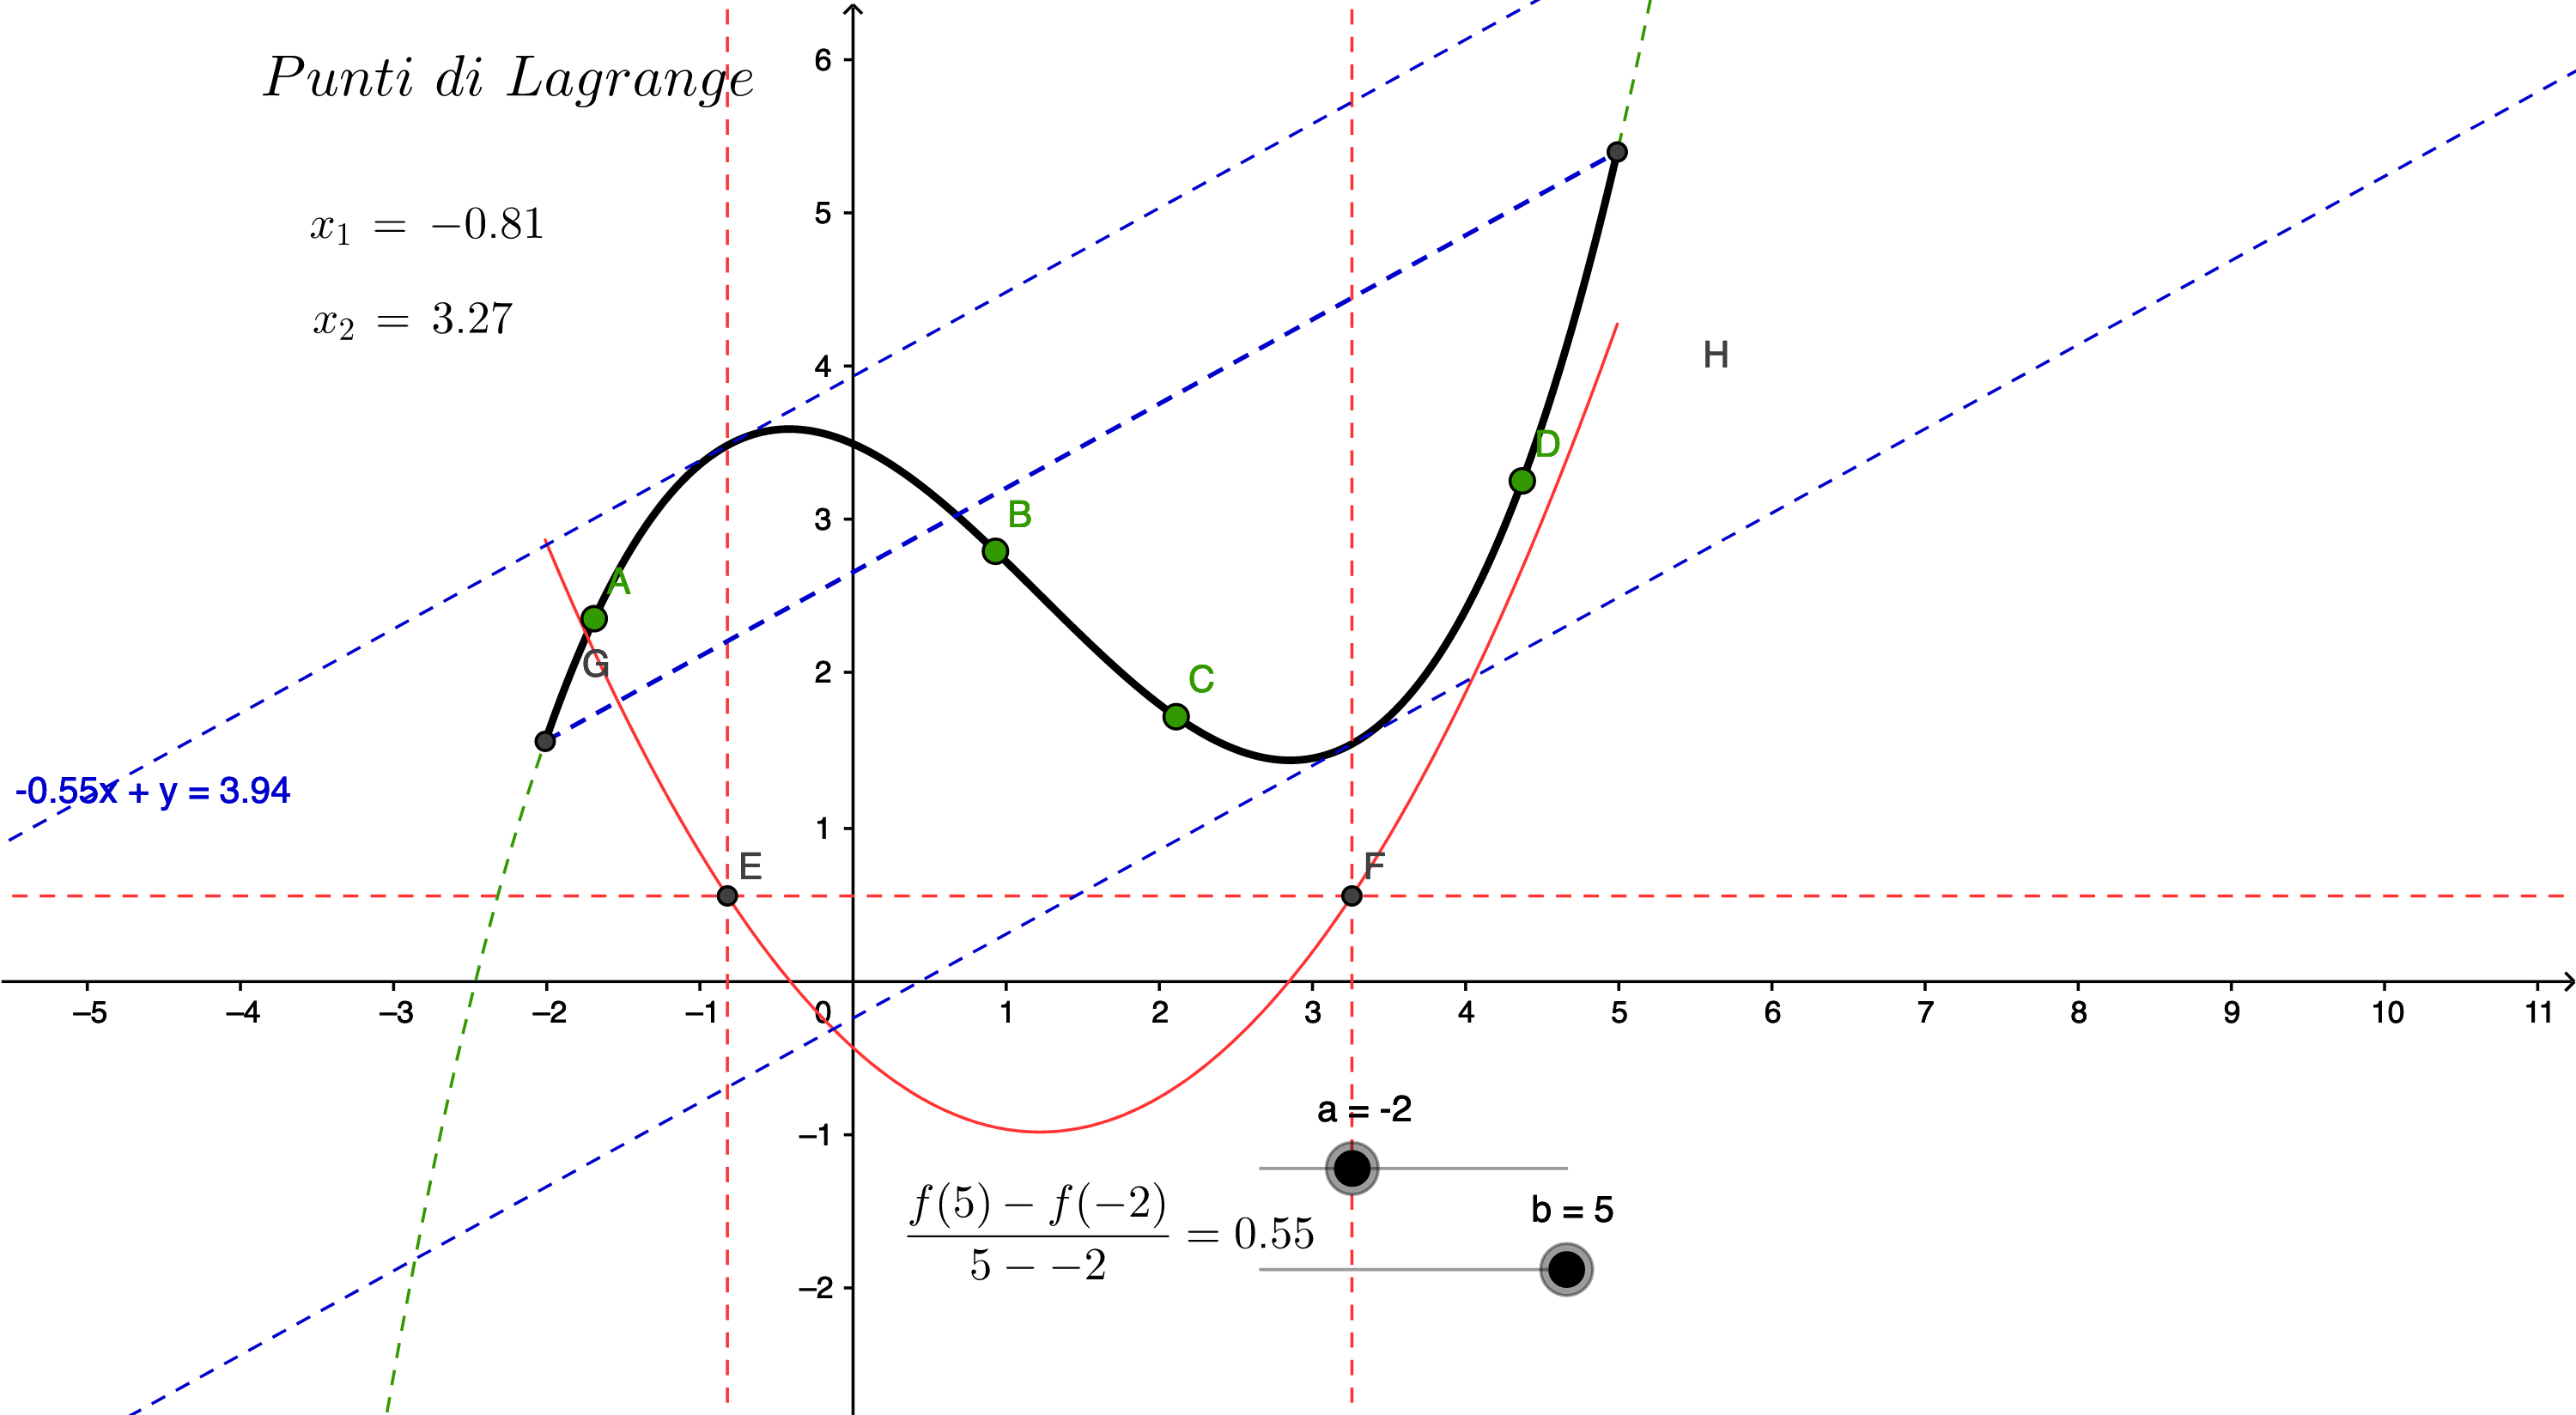
\includegraphics{Lagrange}
\end{frame}

\begin{frame}
\begin{alertblock}{Block Title}
Lorem ipsum dolor sit amet, consectetur adipisicing elit, 
sed do eiusmod tempor incididunt ut labore et 
dolore magna aliqua.
\end{alertblock}

\begin{definition}
A prime number is a number that...
\end{definition}

\begin{example}
Lorem ipsum dolor sit amet, consectetur adipisicing elit, 
sed do eiusmod tempor incididunt ut labore et
dolore magna aliqua.
\end{example}
\end{frame}

\begin{frame}
\begin{theorem}[Pythagoras] 
$ a^2 + b^2 = c^2$
\end{theorem}

\begin{corollary}
$ x + y = y + x  $
\end{corollary}
\begin{proof}
$\omega +\phi = \epsilon $
\end{proof}
\end{frame}

\section{Compiti per casa}

\begin{frame}[t]{Esercizi sulle derivate}

\begin{alertblock}{cosa studiare} \vspace{2pt}
Lorem ipsum dolor sit amet, consectetur adipisicing elit, 
sed do eiusmod tempor incididunt ut labore et 
dolore magna aliqua.
\end{alertblock}

\begin{alertblock}{come studiare} \vspace{2pt}
Lorem ipsum dolor sit amet, consectetur adipisicing elit, 
sed do eiusmod tempor incididunt ut labore et 
dolore magna aliqua.
\end{alertblock}

\begin{alertblock}{esrcizi - revisione} \vspace{2pt}
Lorem ipsum dolor sit amet, consectetur adipisicing elit, 
sed do eiusmod tempor incididunt ut labore et 
dolore magna aliqua.
\end{alertblock}

\begin{alertblock}{nuovi esercizi} \vspace{2pt}
Lorem ipsum dolor sit amet, consectetur adipisicing elit, 
sed do eiusmod tempor incididunt ut labore et 
dolore magna aliqua.
\end{alertblock}
\end{frame}

\end{document}